\subsection{Design du système}
    Le système se découpe essentiellement en 3 parties:
    \begin{itemize}
        \item[-] Coté utilisateur
        \item[-] Coté jeu
        \item[-] Coté serveur
    \end{itemize}
    \subsubsection{Coté utilisateur}
        % \makebox[\textwidth]{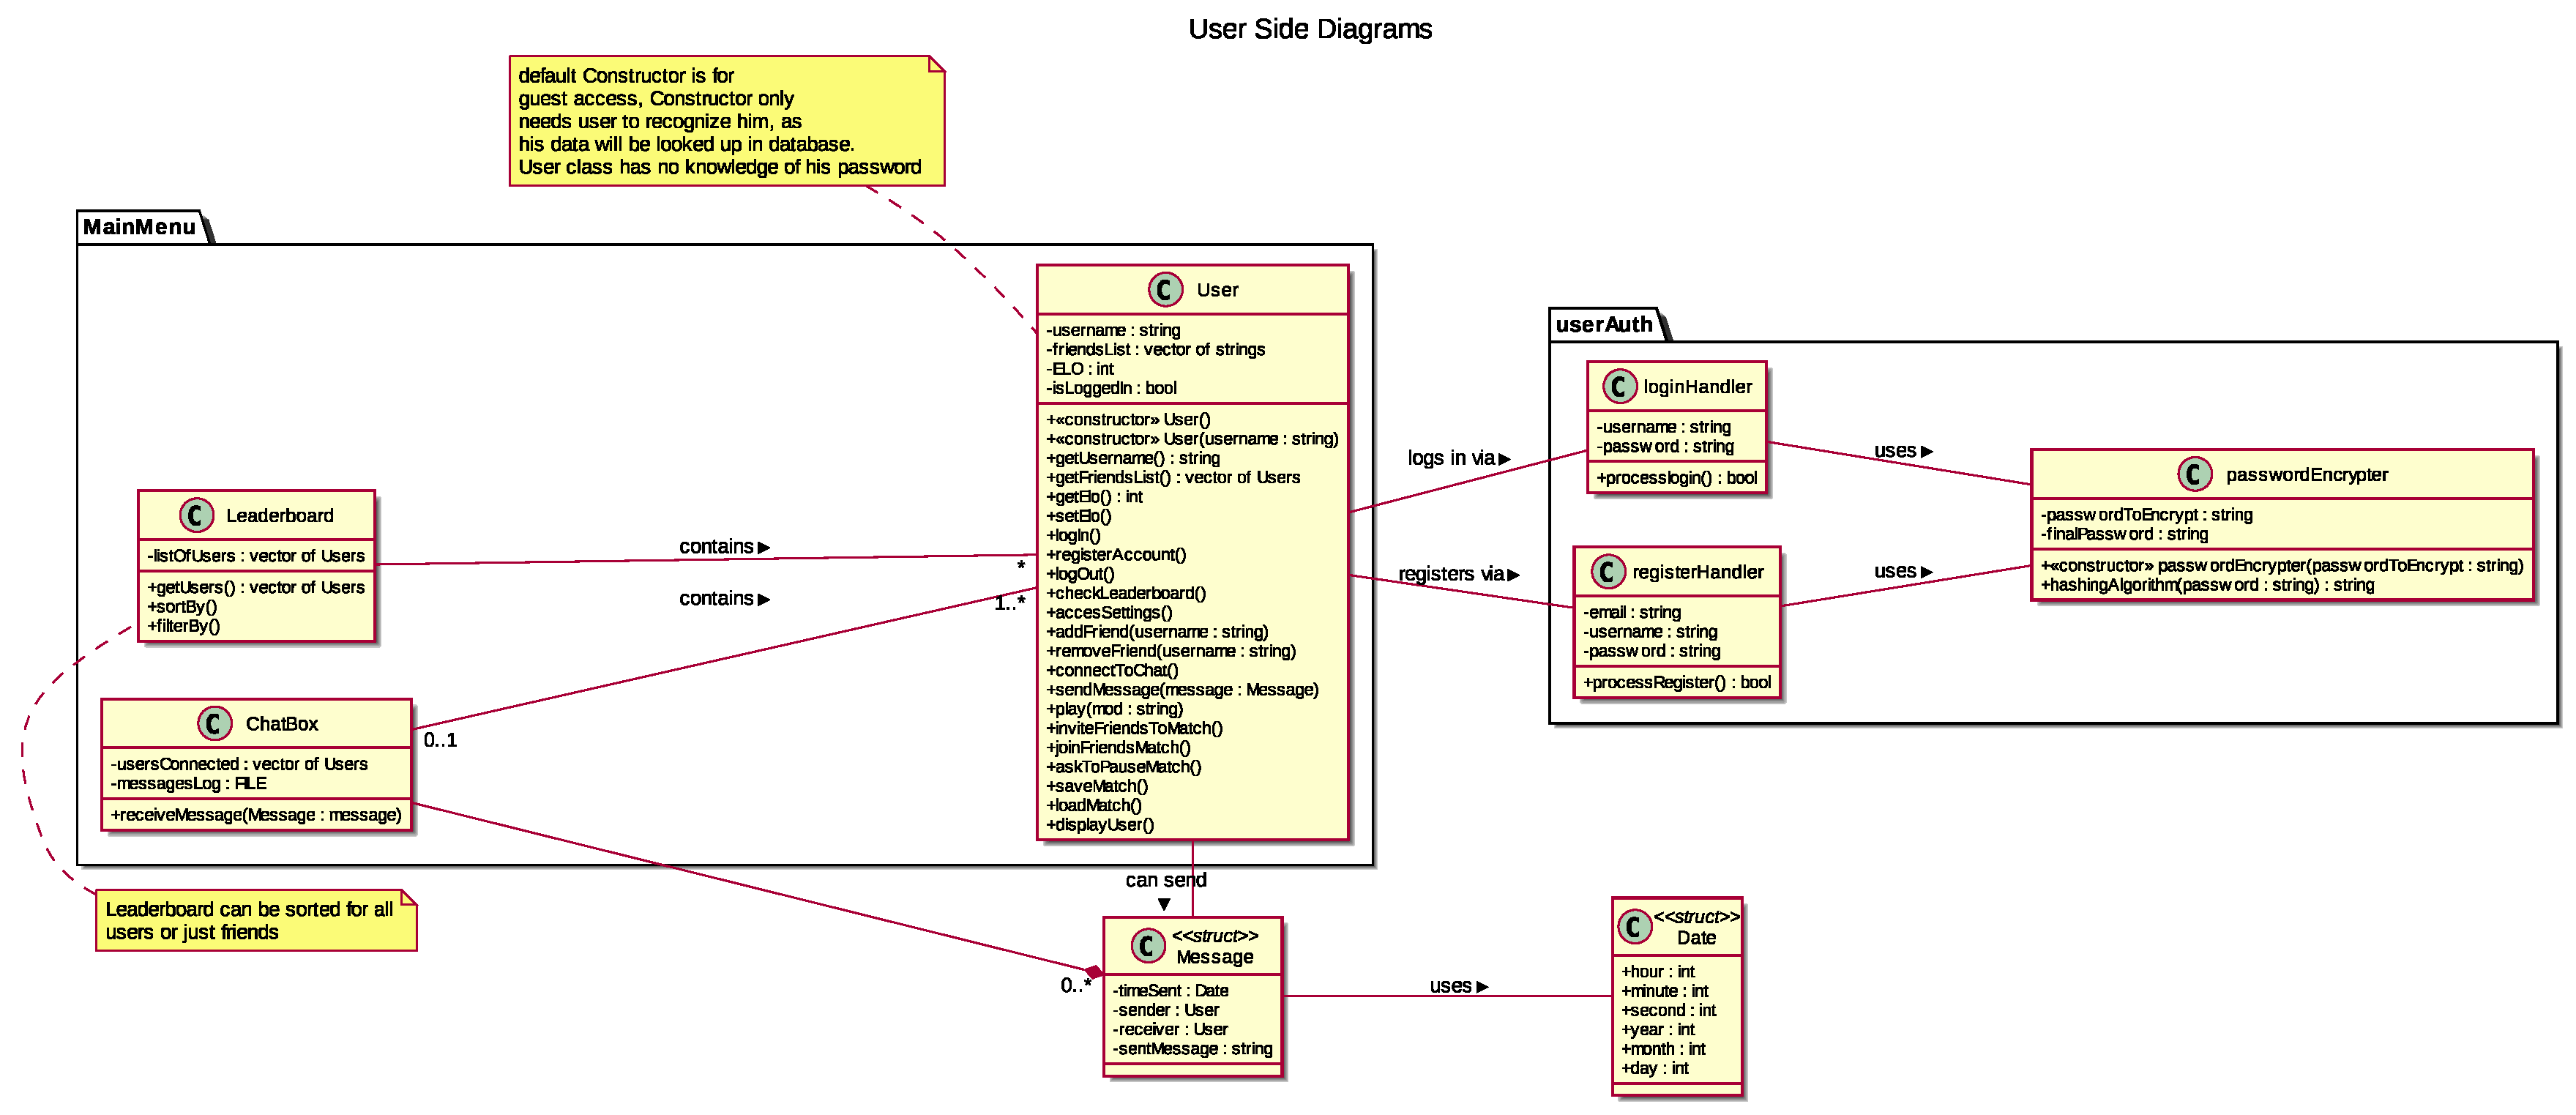
\includegraphics[width=\textwidth]{UserSideDiagrams.eps}}
    \addimg{img/6_UserSideDiagrams.eps}{width=\textwidth}{Diagrammes du côté utilisateur}{usrside}
        L'utilisateur entre dans l'application en tant que \textit{guest} mais ne peut pas jouer.
        Pour pouvoir lancer une partie, l'utilisateur doit tout d'abord se connecter à son compte ou en créer un s'il n'en a pas. Ces deux évènements se feront à travers des "handlers", qui géreront les requêtes en passant à travers la base de données et le serveur. Une fois connecté.e, l'utilisateur aura accès à toutes les fonctionnalités qu'offre le logiciel (cfr. Sections 2 et 4).
    \subsubsection{Coté jeu}
        % \makebox[\textwidth]{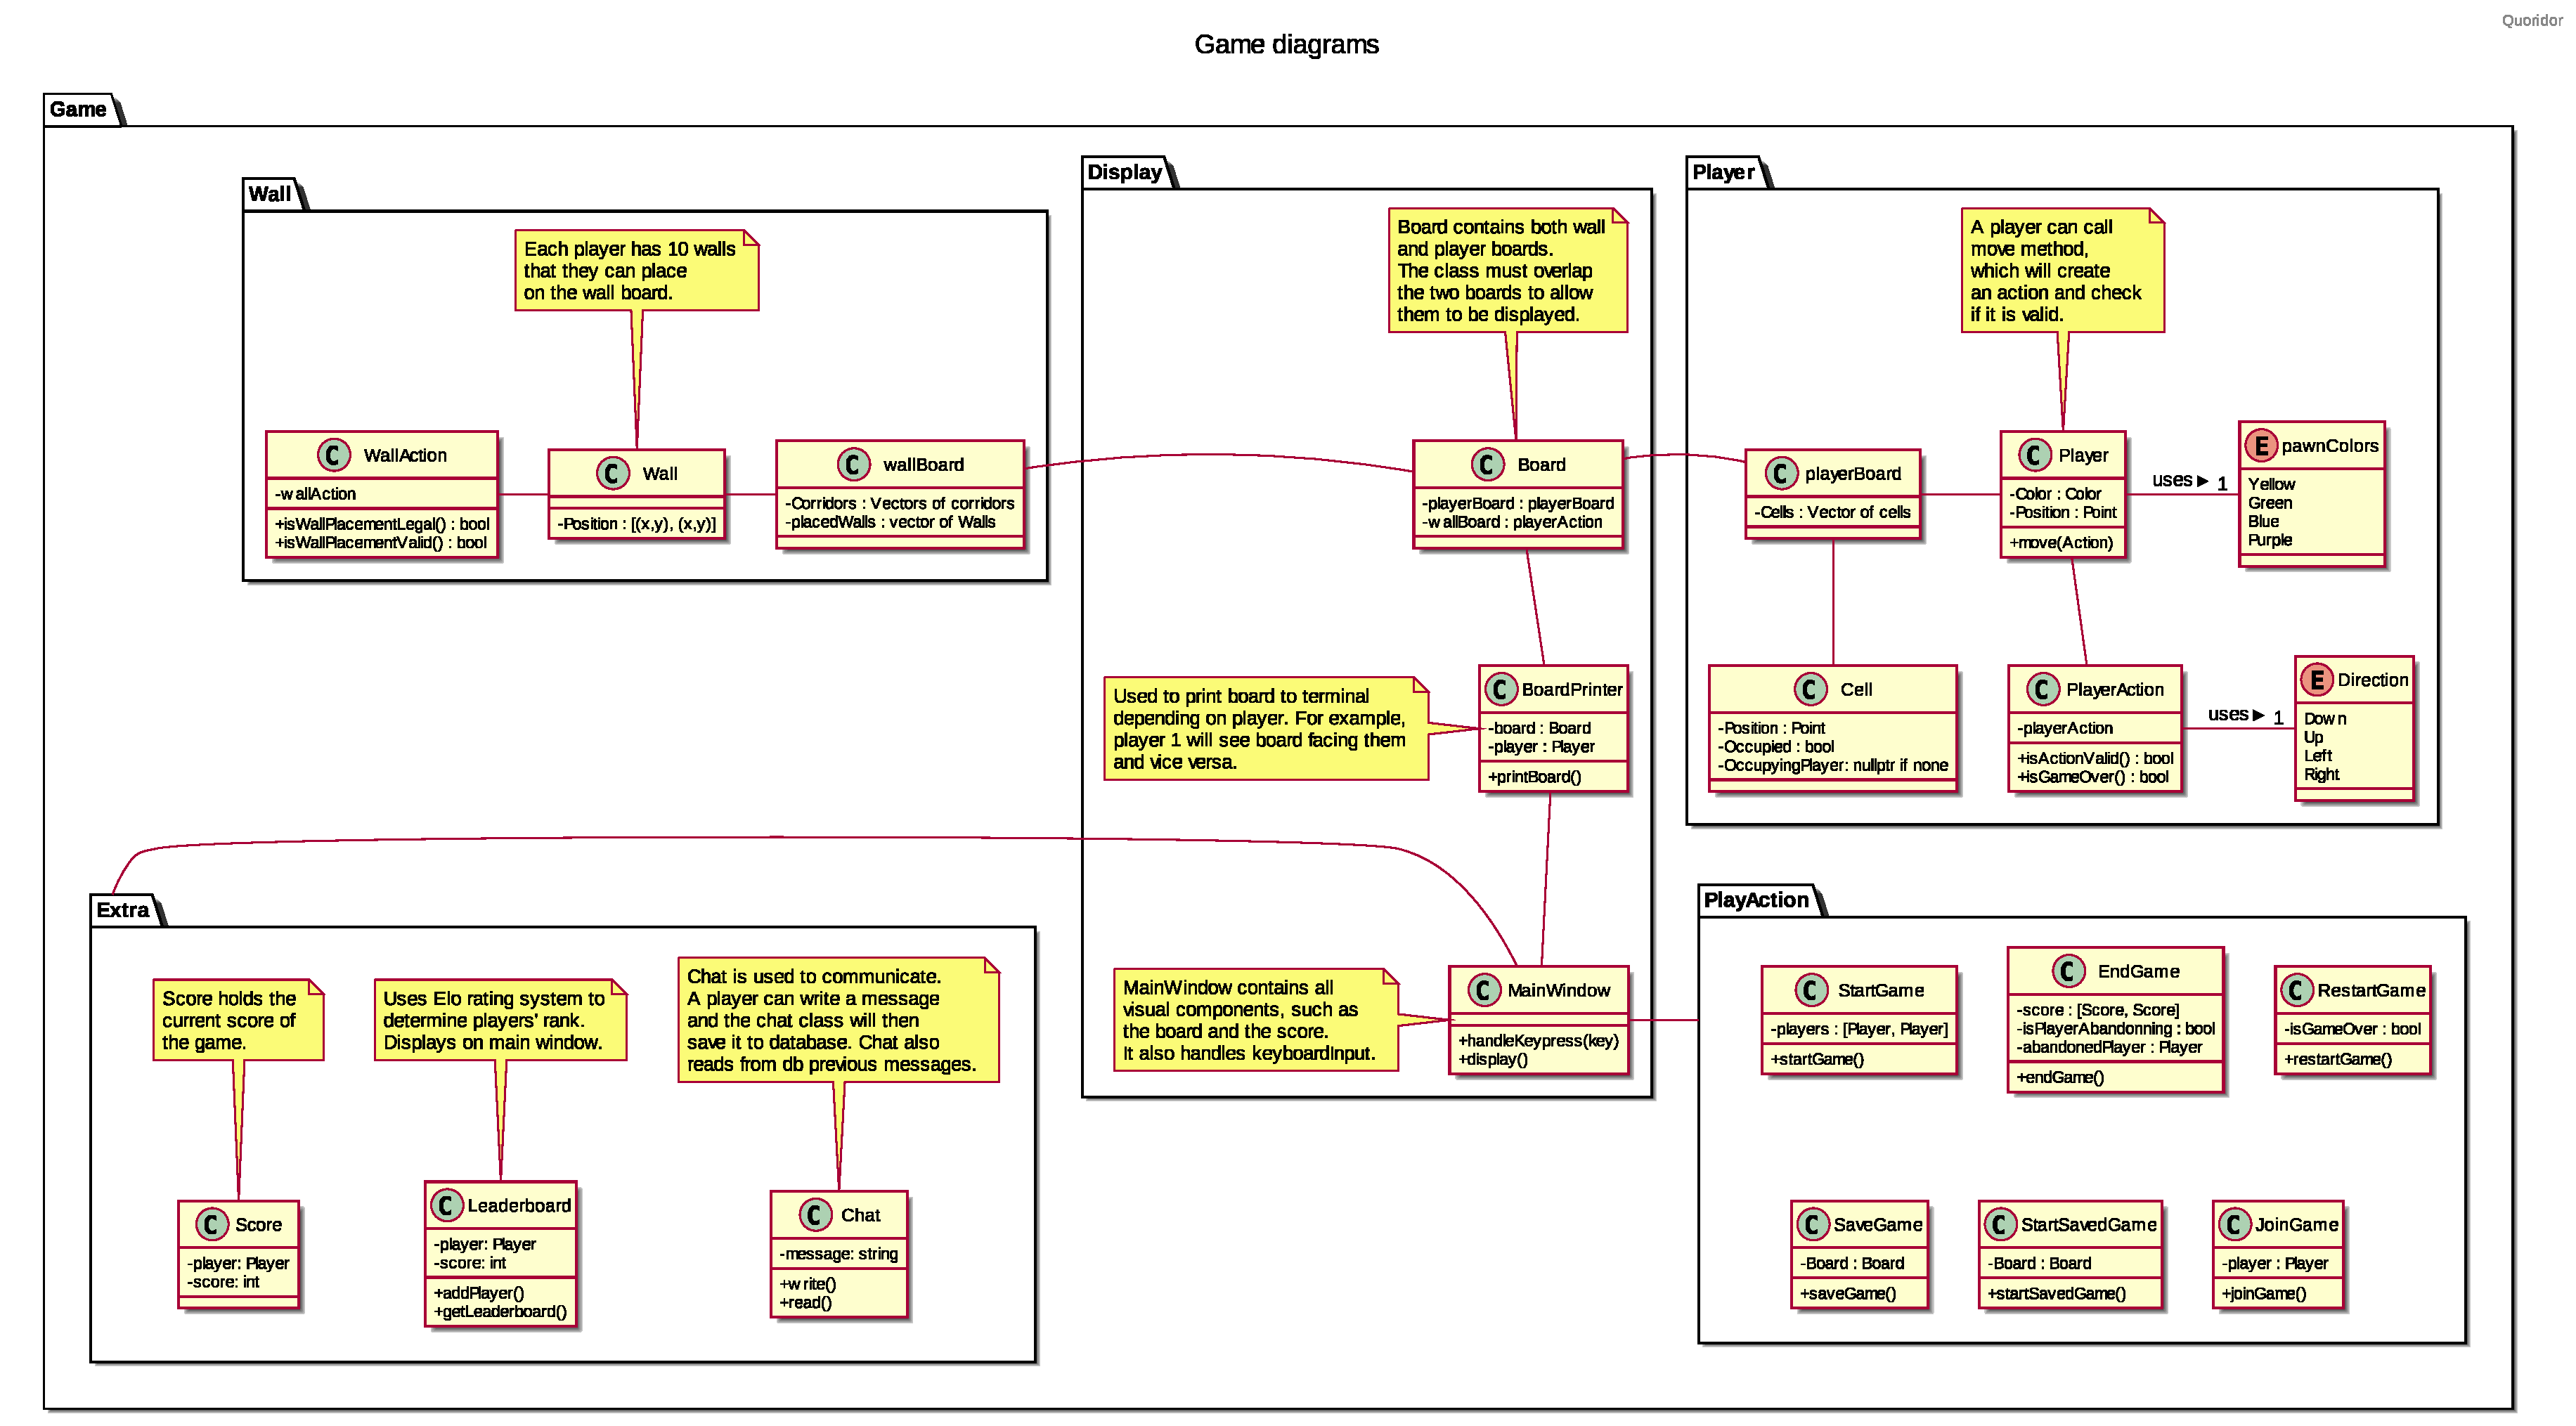
\includegraphics[width=\textwidth]{GameDiagrams.eps}}
    \addimg{img/6_GameDiagrams.eps}{width=\textwidth}{Diagrammes de jeu}{gameside}
        Le jeu est divisé en deux plateaux. Le plateau mur (\textit{WallBoard}) contient les murs. Tandis que le plateau joueur contient les pions des joueurs. Chaque pion a une couleur différente ce qui permet aux joueurs de se distinguer l'un de l'autre. La classe \textit{Board} a pour but de combiner chaque plateau pour ensuite les afficher via \textit{BoardPrinter} dans \textit{MainWindow}.

        Le \textit{PlayerBoard} est divisé en cases. Chaque case peut accueillir au maximum un pion définit par la classe \textit{Player}. Chaque \textit{Player} peut se déplacer sur le \textit{PlayerBoard} en faisant appel à la classe \textit{PlayerAction} qui va vérifier si le coup est valide avant de déplacer le pion sur le \textit{PlayerBoard}.

        Le \textit{WallBoard} est quant à lui divisé en couloir. Chaque couloir peut contenir un mur. Un couloir a une largeur de 2 cases.
        L'utilisateur peut placer un mur en faisant appel à \textit{WallAction} qui va d'abord vérifier si l'action est valide avant de placer le mur sur le \textit{WallBoard}.
